\begin{definicja}
  Niech \(\to\) będzie relacją binarną w zbiorze \(A\). 
\begin{enumerate}
  \setlength\itemsep{0em}
  \item[(CR) ] Powiemy, że \(\to\) ma \emph{własność Churcha-Rossera}, jeśli
               dla dowolnych \(a,\,b,\,c\in A\) takich, że
               \(a\to^{*}b\) oraz \(a\to^{*} c\) istnieje \(d\in A\)
               takie, że \(b\to^{*} d\) i \(c\to^{*} d\).

  \item[(WCR)] Powiemy, że \(\to\) ma \emph{słabą własność 
               Churcha-Rossera}a, jesli dla dowolnych \(a,\,b,\,c\in A\)
               takich, że \(a\to b\) oraz \(a\to c\) istnieje \(d\in A\) 
               takie, że \(b\to^{*} d\) i \(c\to^{*} d\).
\end{enumerate}
\end{definicja}
\begin{uwaga*}
  Rozważmy następujący graf skierowany, w którym krawdzie odpowiadają relacji \(\to\) w zbiorze \(\{a,b,c,d\}\):
  \begin{figure}[h]
    \centering
    \includegraphics[width=0.32\linewidth]{../wcrnotcr_example}
  \end{figure}

  Widzimy, że relacja \(\to\) ma własnosność WCR, ale nie ma własności CR.
\end{uwaga*}
\begin{definicja}(Postać normalna)
  Powiemy, że \(x\in A\) jest \emph{redukowalny}, jeśli istnieje \(y\in A\) takie, że \(x\to y\). W przeciwnym wypadku powiemy, że \(x\) jest w \emph{postaci normalnej} i będziemy pisali \(x\in\mathrm{NF}\). 
  
  Element \(y\in A\) nazywamy \emph{postacią normalną} \(x\in A\), jesli \(x\to^{*}y\) i \(y\in\mathrm{NF}\). Jeśli \(y\) jest postacią normalną \(x\) i \(y\) jest jedyną postacią normalną \(x\), to piszemy \(x\downarrow y\). W przeciwnym wypadku, czyli jeśli istnieją \(y, z\in \mathrm{NF}, y\neq z\) takie, że \(x\to^{*} y\) i \(x\to^{*} z\), powiemy, że \(x\) jest \emph{niejednoznaczny}. 
\end{definicja}

\begin{definicja}(Własność silnej normalizacji)
  Powiemy, że relacja \(\to\) jest \emph{silnie normalizowalna} (ma własność SN, od ang. \emph{strong normalizable}), jeśli nie istnieje nieskończony ciąg redukcji \(a_0 \to a_1 \to a_2 \to \dots\)
\end{definicja}

\begin{twierdzenie}(Lemat Newmana)\label{thm:newman_lemma}
Niech \(\to\) bedzie relacją binarną mającą własność SN. Jeśli \(\to\) ma własność WCR, to \(\to\) ma własność CR.
\end{twierdzenie}
\begin{dowod}


Niech \(\to\) będzie relacją binarną na \(A\) o własności SN i WCR. Ponieważ \(\to\) jest SN, to każdy \(a\) jest normalizowalny. Rozważmy następujące przypadki:

\begin{minipage}{.75\textwidth}
\begin{enumerate}[label={\roman*)}, ref={\roman*)}]
  \setlength\itemsep{0em}
  \item Niech \(a\in A\). Jeśli \(a\) nie jest niejednoznaczny, to teza zachodzi.
  \item
      Przypuśćmy, że \(a\) jest niejednoznaczny. wówczas istnieje inny \(a'\in A\), który też jest niejednoznaczny oraz \(a\to a'\). Istotnie, przypuśćmy, że \(a\to^{*} b_1\), \(a \to^{*} b_2\) i niech \(b_1\) i \(b_2\) będą różnymi postaciami normalnymi. Ponieważ \(b_1\) i \(b_2\) są różne, to obydwie te redukcje składają się przynajmniej z jednego kroku. Mają więc postać:
      \begin{align*}
        a \to a_1 \to^{*} b_1 \quad \text{oraz} \quad a\to a_2 \to^{*} b_2
      \end{align*}
    Jeśli \(a_1=a_2\), to \(a'=a_1=a_2\) i wystarczy wybrać \(a'=a_1\).
    Jeśli jednak \(a_1 \neq a_2\), to z własności WCR istnieje
    \(b_3 \in A\) taka, że \(a_1 \to^{*} b_3\) oraz \(a_2 \to^{*} b_3\).
    Z własności SN możemy przyjąć, że \(b_3\) jest w postaci normalnej.

% \begin{figure}[htb]
%   \centering
%   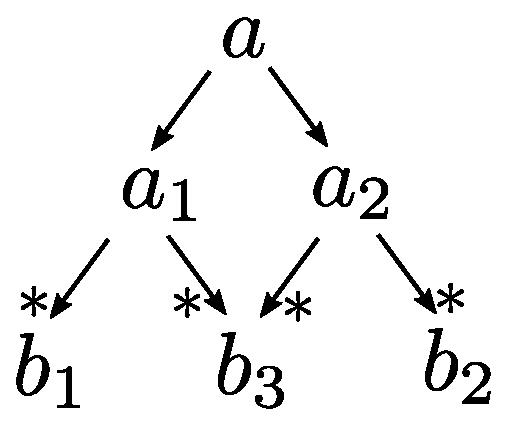
\includegraphics[width=0.195\linewidth]{../newman_3}
%   \caption{}
% \end{figure}
    \vspace{3em}
    Ponieważ \(b_1 \neq b_2\), to albo \(b_1 \neq b_3\), albo \(b_2 \neq b_3\).
    Możemy więc wybrać \(a'=a_1\) lub \(a'=a_2\). Kontynuując tę konstrukcję widzimy, że otrzymujemy nieskończoną redukcję, wbrew założeniu, że \(\to\) ma własność SN.

    Zatem nie istnieją w \(A\) elementy niejednoznaczne.\qed
\end{enumerate}
\end{minipage}
  \begin{minipage}{.25\textwidth}
    \begin{center}
    \vspace{2em}
    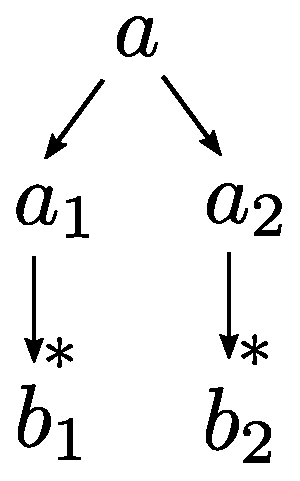
\includegraphics[width=0.41\linewidth]{../newman_1}
    \vspace{4em}

    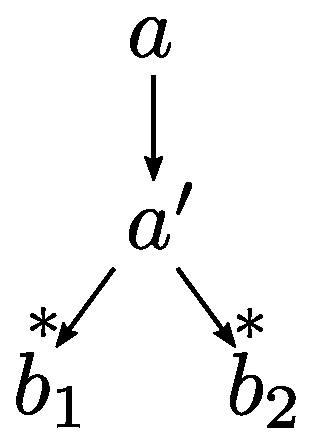
\includegraphics[width=0.41\linewidth]{../newman_2}
    \vspace{3em}

    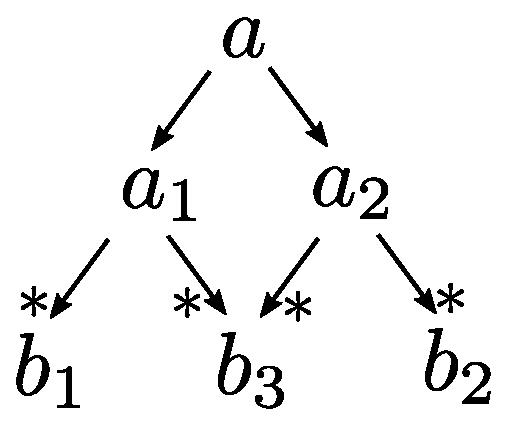
\includegraphics[width=0.71\linewidth]{../newman_3}
    \end{center}
  \end{minipage}
\end{dowod}
